\documentclass{article}\usepackage[]{graphicx}\usepackage[]{color}
%% maxwidth is the original width if it is less than linewidth
%% otherwise use linewidth (to make sure the graphics do not exceed the margin)
\makeatletter
\def\maxwidth{ %
  \ifdim\Gin@nat@width>\linewidth
    \linewidth
  \else
    \Gin@nat@width
  \fi
}
\makeatother

\definecolor{fgcolor}{rgb}{0.345, 0.345, 0.345}
\newcommand{\hlnum}[1]{\textcolor[rgb]{0.686,0.059,0.569}{#1}}%
\newcommand{\hlstr}[1]{\textcolor[rgb]{0.192,0.494,0.8}{#1}}%
\newcommand{\hlcom}[1]{\textcolor[rgb]{0.678,0.584,0.686}{\textit{#1}}}%
\newcommand{\hlopt}[1]{\textcolor[rgb]{0,0,0}{#1}}%
\newcommand{\hlstd}[1]{\textcolor[rgb]{0.345,0.345,0.345}{#1}}%
\newcommand{\hlkwa}[1]{\textcolor[rgb]{0.161,0.373,0.58}{\textbf{#1}}}%
\newcommand{\hlkwb}[1]{\textcolor[rgb]{0.69,0.353,0.396}{#1}}%
\newcommand{\hlkwc}[1]{\textcolor[rgb]{0.333,0.667,0.333}{#1}}%
\newcommand{\hlkwd}[1]{\textcolor[rgb]{0.737,0.353,0.396}{\textbf{#1}}}%

\usepackage{framed}
\makeatletter
\newenvironment{kframe}{%
 \def\at@end@of@kframe{}%
 \ifinner\ifhmode%
  \def\at@end@of@kframe{\end{minipage}}%
  \begin{minipage}{\columnwidth}%
 \fi\fi%
 \def\FrameCommand##1{\hskip\@totalleftmargin \hskip-\fboxsep
 \colorbox{shadecolor}{##1}\hskip-\fboxsep
     % There is no \\@totalrightmargin, so:
     \hskip-\linewidth \hskip-\@totalleftmargin \hskip\columnwidth}%
 \MakeFramed {\advance\hsize-\width
   \@totalleftmargin\z@ \linewidth\hsize
   \@setminipage}}%
 {\par\unskip\endMakeFramed%
 \at@end@of@kframe}
\makeatother

\definecolor{shadecolor}{rgb}{.97, .97, .97}
\definecolor{messagecolor}{rgb}{0, 0, 0}
\definecolor{warningcolor}{rgb}{1, 0, 1}
\definecolor{errorcolor}{rgb}{1, 0, 0}
\newenvironment{knitrout}{}{} % an empty environment to be redefined in TeX

\usepackage{alltt}

\usepackage{hyperref}
\usepackage[T1]{fontenc}
\usepackage{geometry} % to change the page dimensions
\geometry{letterpaper} % or letterpaper (US) or a5paper or....
\geometry{margin=0.75in} % for example, change the margins to 2 inches all round



\IfFileExists{upquote.sty}{\usepackage{upquote}}{}
\begin{document}

\title{Introduction to spatial data analysis with R}
\author{Edgar Dobriban}

\maketitle
  This script presents an introduction to spatial data analysis with R. It is based on Chapters 2 and 9 of our book: \textbf{Applied Spatial Data Analysis with R}, Roger S. Bivand, Edzer Pebesma and V. Gomez-Rubio
   UseR! Series, Springer, 2nd ed. 2013.
   
   Please consult the textbook for more extensive reference, it is a great resource.
   
  Running this script requires that the code and data bundles from the book be unzipped in the same folder as the script. For instance the zip bundle for chapter 2 is available at: 
  \url{http://www.asdar-book.org/data2ed.php?chapter=2}

Similarly, get the zip bundle for chapter 9.
 
In the first part of the lecture, we will work with existing spatial data in R. Second we will also understand how to create such data.

Okay, let's get started: clear up the workspace and change directory to where the data is!

\begin{knitrout}
\definecolor{shadecolor}{rgb}{0.969, 0.969, 0.969}\color{fgcolor}\begin{kframe}
\begin{alltt}
\hlcom{#set up: clear all  & set wd}
\hlkwd{rm}\hlstd{(}\hlkwc{list}\hlstd{=}\hlkwd{ls}\hlstd{())}
\hlkwd{setwd}\hlstd{(}\hlstr{"C:/Dropbox/253/lat_bundle"}\hlstd{)}
\end{alltt}
\end{kframe}
\end{knitrout}

Let's load two required libraries:

rgdal: processes GDAL - Geospatial Data Analysis files
spdep: Spatial dependence: weighting schemes, statistics and models.

\begin{knitrout}
\definecolor{shadecolor}{rgb}{0.969, 0.969, 0.969}\color{fgcolor}\begin{kframe}
\begin{alltt}
\hlkwd{library}\hlstd{(rgdal)}
\end{alltt}


{\ttfamily\noindent\itshape\color{messagecolor}{\#\# Loading required package: sp\\\#\# rgdal: version: 0.8-16, (SVN revision 498)\\\#\# Geospatial Data Abstraction Library extensions to R successfully loaded\\\#\# Loaded GDAL runtime: GDAL 1.11.0, released 2014/04/16\\\#\# Path to GDAL shared files: C:/Users/Edgar/Documents/R/win-library/3.1/rgdal/gdal\\\#\# GDAL does not use iconv for recoding strings.\\\#\# Loaded PROJ.4 runtime: Rel. 4.8.0, 6 March 2012, [PJ\_VERSION: 480]\\\#\# Path to PROJ.4 shared files: C:/Users/Edgar/Documents/R/win-library/3.1/rgdal/proj}}\begin{alltt}
\hlkwd{library}\hlstd{(spdep)}
\end{alltt}


{\ttfamily\noindent\itshape\color{messagecolor}{\#\# Loading required package: Matrix}}\end{kframe}
\end{knitrout}

The data set consists of Leukemia incidence in 281 census tracts in 8 central NY state counties (and was collected in the 1980's)

This is how we read the data sets:
\begin{knitrout}
\definecolor{shadecolor}{rgb}{0.969, 0.969, 0.969}\color{fgcolor}\begin{kframe}
\begin{alltt}
\hlstd{NY8} \hlkwb{<-} \hlkwd{readOGR}\hlstd{(}\hlstr{"."}\hlstd{,} \hlstr{"NY8_utm18"}\hlstd{)}
\end{alltt}
\begin{verbatim}
## OGR data source with driver: ESRI Shapefile 
## Source: ".", layer: "NY8_utm18"
## with 281 features and 17 fields
## Feature type: wkbPolygon with 2 dimensions
\end{verbatim}
\begin{alltt}
\hlcom{# read Shapefile (spdep package), }
\hlcom{# arguments (1)"." - source: a directory; here current wd }
\hlcom{# (2) layer: shapefile name}
\hlcom{# Note: find shapefiles by googling "[location] shapefile"}
\end{alltt}
\end{kframe}
\end{knitrout}

Some additional data:

\begin{knitrout}
\definecolor{shadecolor}{rgb}{0.969, 0.969, 0.969}\color{fgcolor}\begin{kframe}
\begin{alltt}
\hlcom{#city names}
\hlstd{cities} \hlkwb{<-} \hlkwd{readOGR}\hlstd{(}\hlstr{"."}\hlstd{,} \hlstr{"NY8cities"}\hlstd{)}
\end{alltt}
\begin{verbatim}
## OGR data source with driver: ESRI Shapefile 
## Source: ".", layer: "NY8cities"
## with 6 features and 1 fields
## Feature type: wkbPoint with 2 dimensions
\end{verbatim}
\begin{alltt}
\hlcom{#locations of 11 inactive hazardous waste sites; }
\hlcom{# TCE: Trichloroethylene}
\hlstd{TCE} \hlkwb{<-} \hlkwd{readOGR}\hlstd{(}\hlstr{"."}\hlstd{,} \hlstr{"TCE"}\hlstd{)}
\end{alltt}
\begin{verbatim}
## OGR data source with driver: ESRI Shapefile 
## Source: ".", layer: "TCE"
## with 11 features and 5 fields
## Feature type: wkbPoint with 2 dimensions
\end{verbatim}
\end{kframe}
\end{knitrout}


Let's look at how the data is stored.

\begin{knitrout}
\definecolor{shadecolor}{rgb}{0.969, 0.969, 0.969}\color{fgcolor}\begin{kframe}
\begin{alltt}
\hlcom{# How is the data stored?}
\hlkwd{class}\hlstd{(NY8)}
\end{alltt}
\begin{verbatim}
## [1] "SpatialPolygonsDataFrame"
## attr(,"package")
## [1] "sp"
\end{verbatim}
\begin{alltt}
\hlkwd{getClass}\hlstd{(}\hlstr{"SpatialPolygonsDataFrame"}\hlstd{)}
\end{alltt}
\begin{verbatim}
## Class "SpatialPolygonsDataFrame" [package "sp"]
## 
## Slots:
##                                           
## Name:         data    polygons   plotOrder
## Class:  data.frame        list     integer
##                               
## Name:         bbox proj4string
## Class:      matrix         CRS
## 
## Extends: 
## Class "SpatialPolygons", directly
## Class "Spatial", by class "SpatialPolygons", distance 2
\end{verbatim}
\begin{alltt}
\hlcom{#it's a SpatialPolygonsDataFrame - a data.frame on polygons}

\hlcom{#spatial polygons contain polygons and Spatial* characteristics}
\hlkwd{getClass}\hlstd{(}\hlstr{"SpatialPolygons"}\hlstd{)}
\end{alltt}
\begin{verbatim}
## Class "SpatialPolygons" [package "sp"]
## 
## Slots:
##                                           
## Name:     polygons   plotOrder        bbox
## Class:        list     integer      matrix
##                   
## Name:  proj4string
## Class:         CRS
## 
## Extends: "Spatial"
## 
## Known Subclasses: "SpatialPolygonsDataFrame"
\end{verbatim}
\end{kframe}
\end{knitrout}

\begin{knitrout}
\definecolor{shadecolor}{rgb}{0.969, 0.969, 0.969}\color{fgcolor}\begin{kframe}
\begin{alltt}
\hlcom{# a polygon is a sequence of closed lines;}
\hlcom{# point coordinates where the first point equals the last }
\hlkwd{getClass}\hlstd{(}\hlstr{"Polygon"}\hlstd{)}
\end{alltt}
\begin{verbatim}
## Class "Polygon" [package "sp"]
## 
## Slots:
##                                               
## Name:    labpt    area    hole ringDir  coords
## Class: numeric numeric logical integer  matrix
## 
## Extends: "Line"
\end{verbatim}
\begin{alltt}
\hlcom{#labpt - label point, centroid of polygon}
\hlcom{# a line is an ordered list of coordinates}
\hlkwd{getClass}\hlstd{(}\hlstr{"Line"}\hlstd{)}
\end{alltt}
\begin{verbatim}
## Class "Line" [package "sp"]
## 
## Slots:
##              
## Name:  coords
## Class: matrix
## 
## Known Subclasses: "Polygon"
\end{verbatim}
\end{kframe}
\end{knitrout}

\begin{knitrout}
\definecolor{shadecolor}{rgb}{0.969, 0.969, 0.969}\color{fgcolor}\begin{kframe}
\begin{alltt}
\hlcom{#finally... Spatial is the mother class of all Spatial* classes }
\hlcom{# used in in the sp package}
\hlkwd{getClass}\hlstd{(}\hlstr{"Spatial"}\hlstd{)}
\end{alltt}
\begin{verbatim}
## Class "Spatial" [package "sp"]
## 
## Slots:
##                               
## Name:         bbox proj4string
## Class:      matrix         CRS
## 
## Known Subclasses: 
## Class "SpatialPoints", directly
## Class "SpatialGrid", directly
## Class "SpatialLines", directly
## Class "SpatialPolygons", directly
## Class "SpatialPointsDataFrame", by class "SpatialPoints", distance 2
## Class "SpatialPixels", by class "SpatialPoints", distance 2
## Class "SpatialGridDataFrame", by class "SpatialGrid", distance 2
## Class "SpatialLinesDataFrame", by class "SpatialLines", distance 2
## Class "SpatialPixelsDataFrame", by class "SpatialPoints", distance 3
## Class "SpatialPolygonsDataFrame", by class "SpatialPolygons", distance 2
\end{verbatim}
\end{kframe}
\end{knitrout}


What does the data contain?
\begin{knitrout}
\definecolor{shadecolor}{rgb}{0.969, 0.969, 0.969}\color{fgcolor}\begin{kframe}
\begin{alltt}
\hlkwd{summary}\hlstd{(NY8)}
\end{alltt}
\begin{verbatim}
## Object of class SpatialPolygonsDataFrame
## Coordinates:
##       min     max
## x  358242  480393
## y 4649755 4808545
## Is projected: TRUE 
## proj4string :
## [+proj=utm +zone=18 +ellps=WGS84 +units=m
## +no_defs]
## Data attributes:
##                   AREANAME          AREAKEY   
##  NA                   : 83   36007000100:  1  
##  Syracuse city        : 63   36007000200:  1  
##  Binghamton city      : 18   36007000300:  1  
##  Remainder of Clay tow:  6   36007000400:  1  
##  Johnson City village :  5   36007000500:  1  
##  Onondaga town        :  5   36007000600:  1  
##  (Other)              :101   (Other)    :275  
##        X                Y         
##  Min.   :-55.48   Min.   :-75.29  
##  1st Qu.:-19.46   1st Qu.:-30.60  
##  Median :-12.47   Median : 31.97  
##  Mean   :-11.31   Mean   :  4.98  
##  3rd Qu.: -1.21   3rd Qu.: 39.12  
##  Max.   : 53.51   Max.   : 56.41  
##                                   
##       POP8          TRACTCAS   
##  Min.   :    9   Min.   :0.00  
##  1st Qu.: 2510   1st Qu.:0.31  
##  Median : 3433   Median :1.89  
##  Mean   : 3764   Mean   :2.11  
##  3rd Qu.: 4889   3rd Qu.:3.08  
##  Max.   :13015   Max.   :9.29  
##                                
##     PROPCAS           PCTOWNHOME    
##  Min.   :0.000000   Min.   :0.0008  
##  1st Qu.:0.000093   1st Qu.:0.4589  
##  Median :0.000413   Median :0.6509  
##  Mean   :0.000595   Mean   :0.5873  
##  3rd Qu.:0.000917   3rd Qu.:0.7561  
##  Max.   :0.006993   Max.   :1.0000  
##                                     
##    PCTAGE65P            Z         
##  Min.   :0.0040   Min.   :-1.921  
##  1st Qu.:0.0999   1st Qu.:-0.717  
##  Median :0.1264   Median :-0.288  
##  Mean   :0.1373   Mean   :-0.216  
##  3rd Qu.:0.1610   3rd Qu.: 0.250  
##  Max.   :0.5051   Max.   : 4.711  
##                                   
##     AVGIDIST       PEXPOSURE         Cases      
##  Min.   :0.018   Min.   :0.613   Min.   :0.000  
##  1st Qu.:0.027   1st Qu.:0.994   1st Qu.:0.309  
##  Median :0.032   Median :1.175   Median :1.889  
##  Mean   :0.149   Mean   :1.804   Mean   :2.107  
##  3rd Qu.:0.130   3rd Qu.:2.566   3rd Qu.:3.083  
##  Max.   :3.526   Max.   :5.865   Max.   :9.286  
##                                                 
##        Xm               Ym        
##  Min.   :-55482   Min.   :-75291  
##  1st Qu.:-19460   1st Qu.:-30601  
##  Median :-12469   Median : 31970  
##  Mean   :-11309   Mean   :  4980  
##  3rd Qu.: -1213   3rd Qu.: 39123  
##  Max.   : 53509   Max.   : 56410  
##                                   
##      Xshift           Yshift       
##  Min.   :363839   Min.   :4653564  
##  1st Qu.:399862   1st Qu.:4698254  
##  Median :406852   Median :4760825  
##  Mean   :408013   Mean   :4733835  
##  3rd Qu.:418108   3rd Qu.:4767978  
##  Max.   :472830   Max.   :4785265  
## 
\end{verbatim}
\begin{alltt}
\hlcom{#Note the special slots of this class}
\hlcom{#Coordinates}
\hlcom{#proj4string}
\hlcom{#Spatial data.frame - with coordinates X,Y}
\end{alltt}
\end{kframe}
\end{knitrout}
What about the 'cities' data?

\begin{knitrout}
\definecolor{shadecolor}{rgb}{0.969, 0.969, 0.969}\color{fgcolor}\begin{kframe}
\begin{alltt}
\hlkwd{summary}\hlstd{(cities)}
\end{alltt}
\begin{verbatim}
## Object of class SpatialPointsDataFrame
## Coordinates:
##               min     max
## coords.x1  372237  445728
## coords.x2 4662141 4771698
## Is projected: TRUE 
## proj4string :
## [+proj=utm +zone=18 +ellps=WGS84 +units=m
## +no_defs]
## Number of points: 6
## Data attributes:
##      Auburn Binghampton    Cortland      Ithaca 
##           1           1           1           1 
##      Oneida    Syracuse 
##           1           1
\end{verbatim}
\end{kframe}
\end{knitrout}

Let's make some plots:

\begin{knitrout}
\definecolor{shadecolor}{rgb}{0.969, 0.969, 0.969}\color{fgcolor}\begin{kframe}
\begin{alltt}
\hlcom{#plot cities & TCE locations}
\hlkwd{plot}\hlstd{(NY8,} \hlkwc{border}\hlstd{=}\hlstr{"grey60"}\hlstd{,} \hlkwc{axes}\hlstd{=}\hlnum{TRUE}\hlstd{)}
\hlkwd{text}\hlstd{(}\hlkwd{coordinates}\hlstd{(cities),} \hlkwc{labels}\hlstd{=}\hlkwd{as.character}\hlstd{(cities}\hlopt{$}\hlstd{names),} \hlkwc{font}\hlstd{=}\hlnum{2}\hlstd{,} \hlkwc{cex}\hlstd{=}\hlnum{1.5}\hlstd{)}
\end{alltt}
\end{kframe}
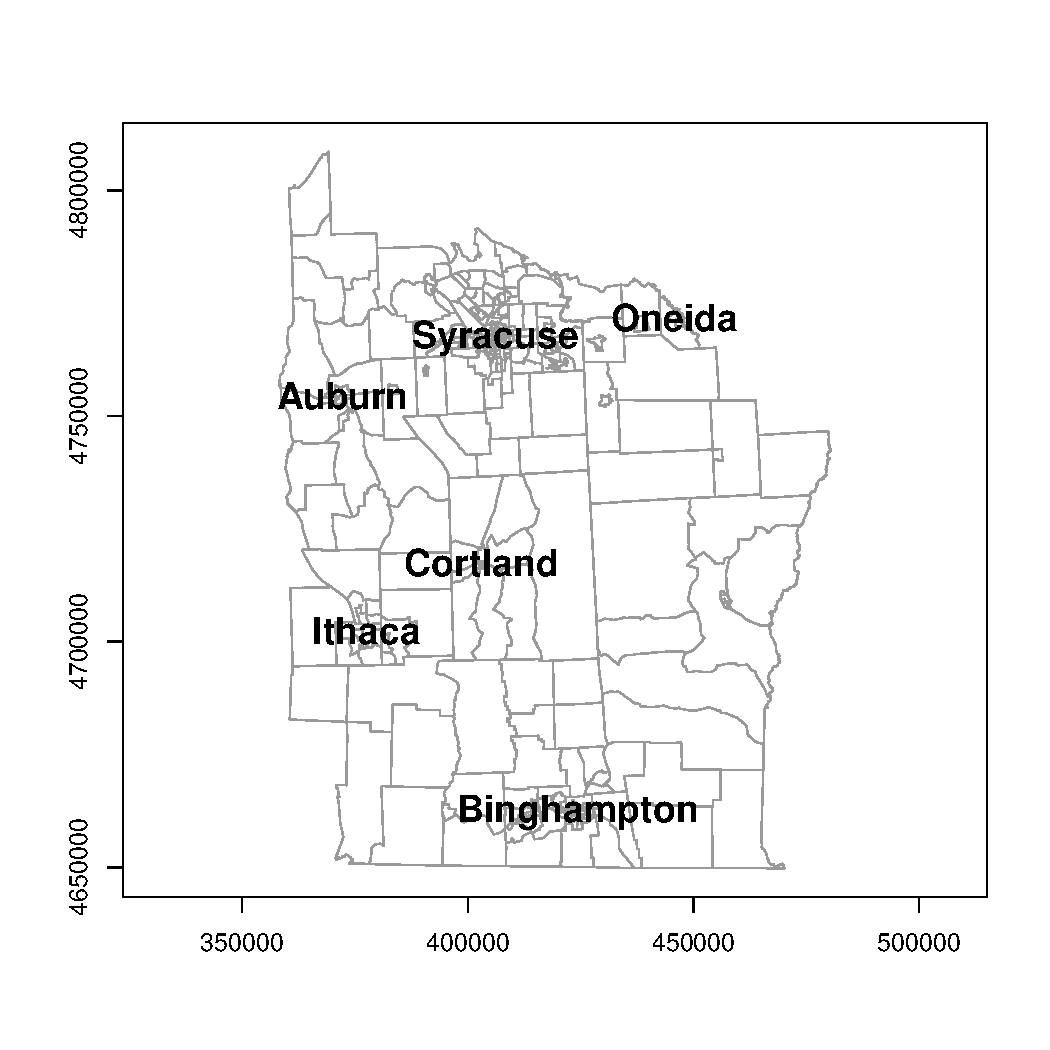
\includegraphics[width=\maxwidth]{figure/unnamed-chunk-101} 
\begin{kframe}\begin{alltt}
\hlkwd{plot}\hlstd{(NY8,} \hlkwc{border}\hlstd{=}\hlstr{"grey60"}\hlstd{,} \hlkwc{axes}\hlstd{=}\hlnum{TRUE}\hlstd{)}
\hlkwd{points}\hlstd{(TCE,} \hlkwc{pch}\hlstd{=}\hlnum{2}\hlstd{,} \hlkwc{cex}\hlstd{=}\hlnum{1.5}\hlstd{)}
\hlkwd{text}\hlstd{(}\hlkwd{coordinates}\hlstd{(TCE),} \hlkwc{labels}\hlstd{=}\hlkwd{as.character}\hlstd{(TCE}\hlopt{$}\hlstd{name),} \hlkwc{cex}\hlstd{=}\hlnum{1.5}\hlstd{,}
     \hlkwc{font}\hlstd{=}\hlnum{1}\hlstd{,} \hlkwc{pos}\hlstd{=}\hlkwd{c}\hlstd{(}\hlnum{4}\hlstd{,}\hlnum{1}\hlstd{,}\hlnum{4}\hlstd{,}\hlnum{1}\hlstd{,}\hlnum{4}\hlstd{,}\hlnum{4}\hlstd{,}\hlnum{4}\hlstd{,}\hlnum{2}\hlstd{,}\hlnum{3}\hlstd{,}\hlnum{4}\hlstd{,}\hlnum{2}\hlstd{),} \hlkwc{offset}\hlstd{=}\hlnum{0.3}\hlstd{)}
\end{alltt}
\end{kframe}
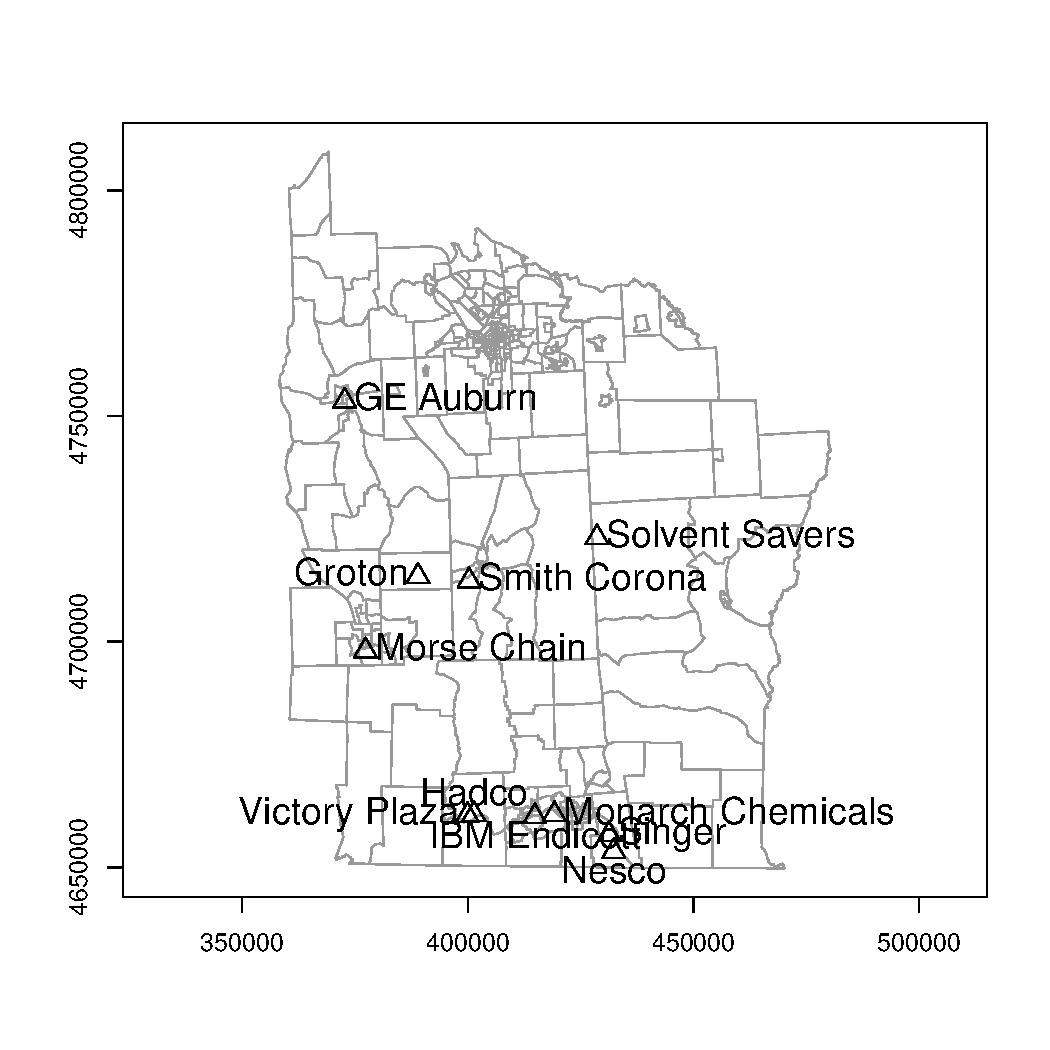
\includegraphics[width=\maxwidth]{figure/unnamed-chunk-102} 

\end{knitrout}

Let's plot one of the features - percent age > 65.

\begin{knitrout}
\definecolor{shadecolor}{rgb}{0.969, 0.969, 0.969}\color{fgcolor}\begin{kframe}
\begin{alltt}
\hlcom{#plot one of the features - percent age > 65}
\hlkwd{spplot}\hlstd{(NY8,} \hlkwd{c}\hlstd{(}\hlstr{"PCTAGE65P"}\hlstd{))}\hlcom{#, col="transparent"}
\end{alltt}
\end{kframe}
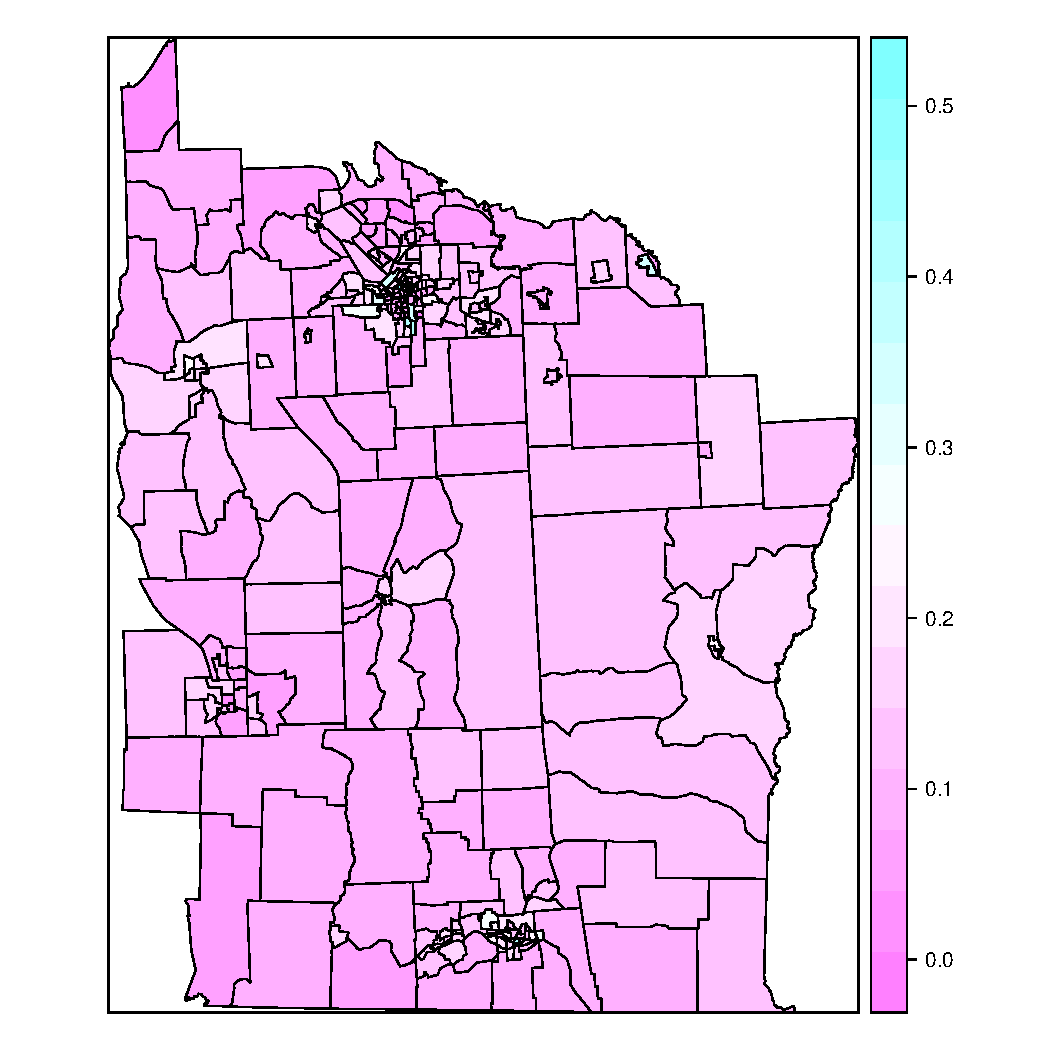
\includegraphics[width=\maxwidth]{figure/unnamed-chunk-111} 
\begin{kframe}\begin{alltt}
\hlkwd{spplot}\hlstd{(NY8,} \hlkwd{c}\hlstd{(}\hlstr{"PCTAGE65P"}\hlstd{),} \hlkwc{col}\hlstd{=}\hlstr{"transparent"}\hlstd{)}
\end{alltt}
\end{kframe}
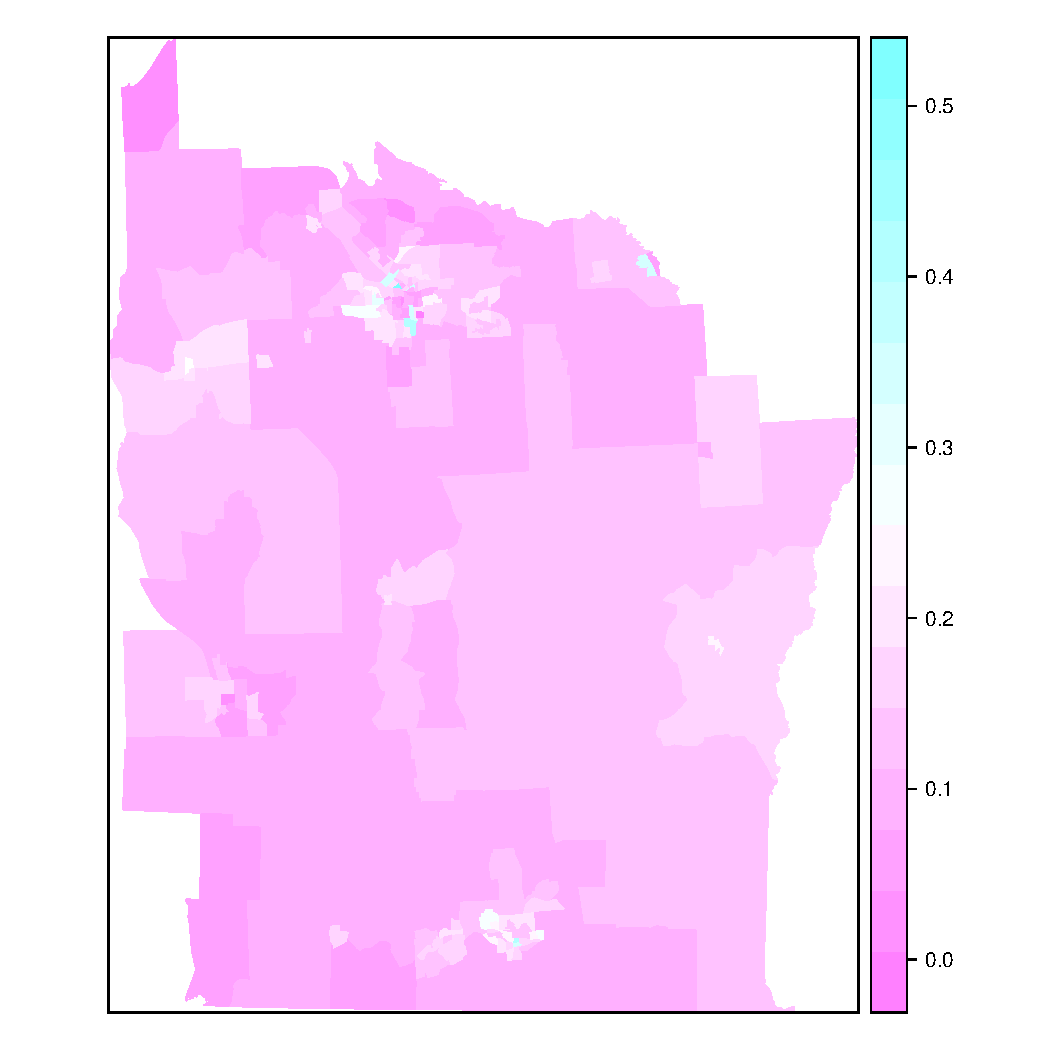
\includegraphics[width=\maxwidth]{figure/unnamed-chunk-112} 

\end{knitrout}


Let's make a different plot, with a  new color palette:
\begin{knitrout}
\definecolor{shadecolor}{rgb}{0.969, 0.969, 0.969}\color{fgcolor}\begin{kframe}
\begin{alltt}
\hlcom{#different plot: new color palette}
\hlcom{#load package}
\hlkwd{library}\hlstd{(}\hlstr{"RColorBrewer"}\hlstd{)}

\hlcom{#color palette creator function}
\hlstd{rds} \hlkwb{<-} \hlkwd{colorRampPalette}\hlstd{(}\hlkwd{brewer.pal}\hlstd{(}\hlnum{8}\hlstd{,} \hlstr{"RdBu"}\hlstd{))}
\hlcom{#get a range for the values}
\hlstd{tr_at} \hlkwb{<-} \hlkwd{seq}\hlstd{(}\hlkwd{min}\hlstd{(NY8}\hlopt{$}\hlstd{PCTAGE65P),} \hlkwd{max}\hlstd{(NY8}\hlopt{$}\hlstd{PCTAGE65P),} \hlkwc{length.out}\hlstd{=}\hlnum{20}\hlstd{)}
\hlcom{#create a color interpolating function taking the required}
\hlcom{#number of shades as argument}
\hlstd{tr_rds} \hlkwb{<-} \hlkwd{rds}\hlstd{(}\hlnum{20}\hlstd{)}
\hlcom{#parameters}
\hlcom{# at - at which values colors change}
\hlcom{# col.regions - specify fill colors }
\hlstd{tr_pl} \hlkwb{<-} \hlkwd{spplot}\hlstd{(NY8,} \hlkwd{c}\hlstd{(}\hlstr{"PCTAGE65P"}\hlstd{),} \hlkwc{at}\hlstd{=tr_at,} \hlkwc{col}\hlstd{=}\hlstr{"transparent"}\hlstd{,}
                \hlkwc{col.regions}\hlstd{=tr_rds,} \hlkwc{main}\hlstd{=}\hlkwd{list}\hlstd{(}\hlkwc{label}\hlstd{=}\hlstr{"Age>65"}\hlstd{,} \hlkwc{cex}\hlstd{=}\hlnum{0.8}\hlstd{))}
\hlkwd{plot}\hlstd{(tr_pl)}
\end{alltt}
\end{kframe}
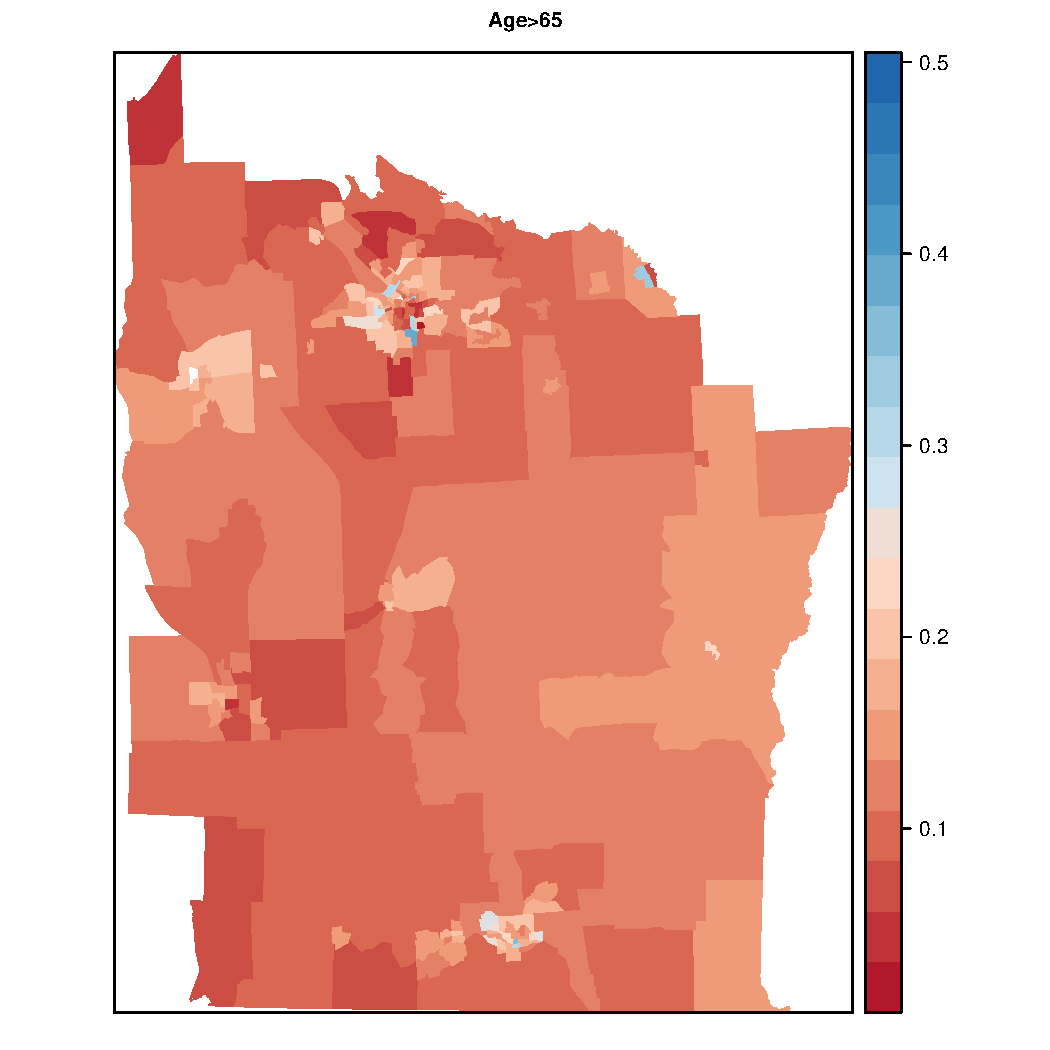
\includegraphics[width=\maxwidth]{figure/unnamed-chunk-12} 

\end{knitrout}

Finally, let's read the last piece of data - a list of neighbors that specifies the lattice structure.

\begin{knitrout}
\definecolor{shadecolor}{rgb}{0.969, 0.969, 0.969}\color{fgcolor}\begin{kframe}
\begin{alltt}
\hlcom{# reads a GAL lattice file into a neighbors list }
\hlstd{NY_nb} \hlkwb{<-} \hlkwd{read.gal}\hlstd{(}\hlstr{"NY_nb.gal"}\hlstd{,} \hlkwc{region.id}\hlstd{=}\hlkwd{row.names}\hlstd{(NY8))}

\hlkwd{summary}\hlstd{(NY_nb)} \hlcom{#which states are neighbors?}
\end{alltt}
\begin{verbatim}
## Neighbour list object:
## Number of regions: 281 
## Number of nonzero links: 1522 
## Percentage nonzero weights: 1.928 
## Average number of links: 5.416 
## Link number distribution:
## 
##  1  2  3  4  5  6  7  8  9 10 11 
##  6 11 28 45 59 49 45 23 10  3  2 
## 6 least connected regions:
## 55 97 100 101 244 245 with 1 link
## 2 most connected regions:
## 34 82 with 11 links
\end{verbatim}
\end{kframe}
\end{knitrout}

\begin{knitrout}
\definecolor{shadecolor}{rgb}{0.969, 0.969, 0.969}\color{fgcolor}\begin{kframe}
\begin{alltt}
\hlkwd{plot}\hlstd{(NY8,} \hlkwc{border}\hlstd{=}\hlstr{"grey60"}\hlstd{,} \hlkwc{axes}\hlstd{=}\hlnum{TRUE}\hlstd{)}
\hlkwd{plot}\hlstd{(NY_nb,} \hlkwd{coordinates}\hlstd{(NY8),} \hlkwc{pch}\hlstd{=}\hlnum{19}\hlstd{,} \hlkwc{cex}\hlstd{=}\hlnum{0.6}\hlstd{,} \hlkwc{add}\hlstd{=}\hlnum{TRUE}\hlstd{)}
\end{alltt}
\end{kframe}
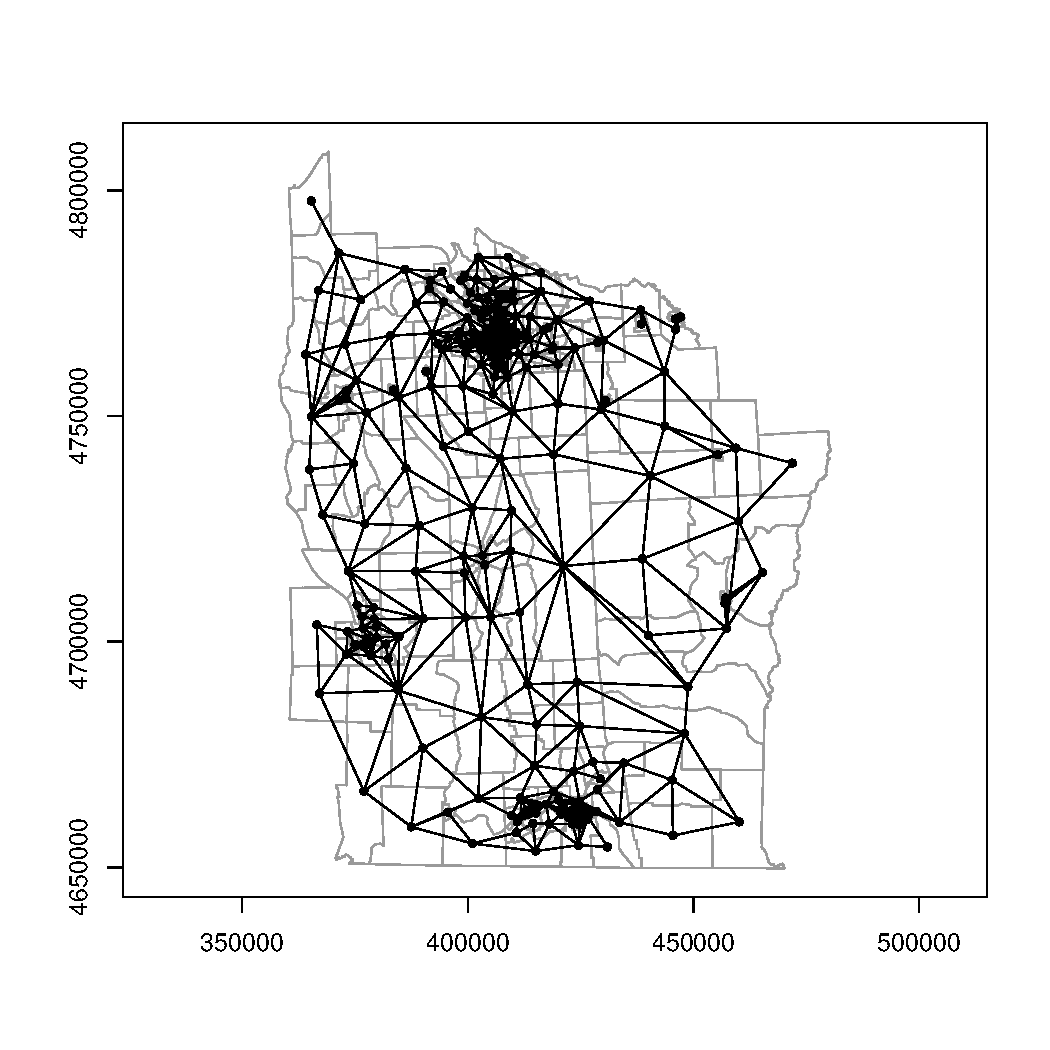
\includegraphics[width=\maxwidth]{figure/unnamed-chunk-14} 

\end{knitrout}


We finally get to the data analysis part! 

Let's first fit a simple linear model, where we regress the leukemia incidence on covariates of interest.

The leukemia incidence is transformed the following way:

$$ z = log(1000(Y_i+1)/n_i) $$

The covariates are:
\begin{itemize}
\item exposure to TCE- log inverse distance from nearest site
\item percent aged >65
\item percent owning home
\end{itemize}

\begin{knitrout}
\definecolor{shadecolor}{rgb}{0.969, 0.969, 0.969}\color{fgcolor}\begin{kframe}
\begin{alltt}
\hlstd{nylm} \hlkwb{<-} \hlkwd{lm}\hlstd{(Z}\hlopt{~}\hlstd{PEXPOSURE}\hlopt{+}\hlstd{PCTAGE65P}\hlopt{+}\hlstd{PCTOWNHOME,} \hlkwc{data}\hlstd{=NY8)}
\hlkwd{summary}\hlstd{(nylm)}
\end{alltt}
\begin{verbatim}
## 
## Call:
## lm(formula = Z ~ PEXPOSURE + PCTAGE65P + PCTOWNHOME, data = NY8)
## 
## Residuals:
##    Min     1Q Median     3Q    Max 
## -1.742 -0.396 -0.033  0.335  4.140 
## 
## Coefficients:
##             Estimate Std. Error t value Pr(>|t|)
## (Intercept)  -0.5173     0.1586   -3.26   0.0012
## PEXPOSURE     0.0488     0.0351    1.39   0.1648
## PCTAGE65P     3.9509     0.6055    6.53  3.2e-10
## PCTOWNHOME   -0.5600     0.1703   -3.29   0.0011
##                
## (Intercept) ** 
## PEXPOSURE      
## PCTAGE65P   ***
## PCTOWNHOME  ** 
## ---
## Signif. codes:  
## 0 '***' 0.001 '**' 0.01 '*' 0.05 '.' 0.1 ' ' 1
## 
## Residual standard error: 0.657 on 277 degrees of freedom
## Multiple R-squared:  0.193,	Adjusted R-squared:  0.184 
## F-statistic: 22.1 on 3 and 277 DF,  p-value: 7.31e-13
\end{verbatim}
\end{kframe}
\end{knitrout}

Let's plot the fit and residual.

\begin{knitrout}
\definecolor{shadecolor}{rgb}{0.969, 0.969, 0.969}\color{fgcolor}\begin{kframe}
\begin{alltt}
\hlstd{NY8}\hlopt{$}\hlstd{lm_fit} \hlkwb{<-} \hlstd{nylm}\hlopt{$}\hlstd{fit}
\hlstd{NY8}\hlopt{$}\hlstd{lm_residual} \hlkwb{<-} \hlstd{nylm}\hlopt{$}\hlstd{residuals}
\hlstd{rds} \hlkwb{<-} \hlkwd{colorRampPalette}\hlstd{(}\hlkwd{brewer.pal}\hlstd{(}\hlnum{8}\hlstd{,} \hlstr{"RdBu"}\hlstd{))}
\hlstd{fit_pl} \hlkwb{<-} \hlkwd{spplot}\hlstd{(NY8,} \hlkwd{c}\hlstd{(}\hlstr{"lm_fit"}\hlstd{),} \hlkwc{col}\hlstd{=}\hlstr{"transparent"}\hlstd{,} \hlkwc{cex}\hlstd{=}\hlnum{0.8}\hlstd{)}
\hlstd{res_pl} \hlkwb{<-} \hlkwd{spplot}\hlstd{(NY8,} \hlkwd{c}\hlstd{(}\hlstr{"lm_residual"}\hlstd{),} \hlkwc{col}\hlstd{=}\hlstr{"transparent"}\hlstd{,} \hlkwc{cex}\hlstd{=}\hlnum{0.8}\hlstd{)}
\hlkwd{plot}\hlstd{(fit_pl,} \hlkwc{split}\hlstd{=}\hlkwd{c}\hlstd{(}\hlnum{1}\hlstd{,}\hlnum{1}\hlstd{,}\hlnum{2}\hlstd{,}\hlnum{1}\hlstd{),} \hlkwc{more}\hlstd{=}\hlnum{TRUE}\hlstd{)}
\hlkwd{plot}\hlstd{(res_pl,} \hlkwc{split}\hlstd{=}\hlkwd{c}\hlstd{(}\hlnum{2}\hlstd{,}\hlnum{1}\hlstd{,}\hlnum{2}\hlstd{,}\hlnum{1}\hlstd{),} \hlkwc{more}\hlstd{=}\hlnum{FALSE}\hlstd{)}
\end{alltt}
\end{kframe}
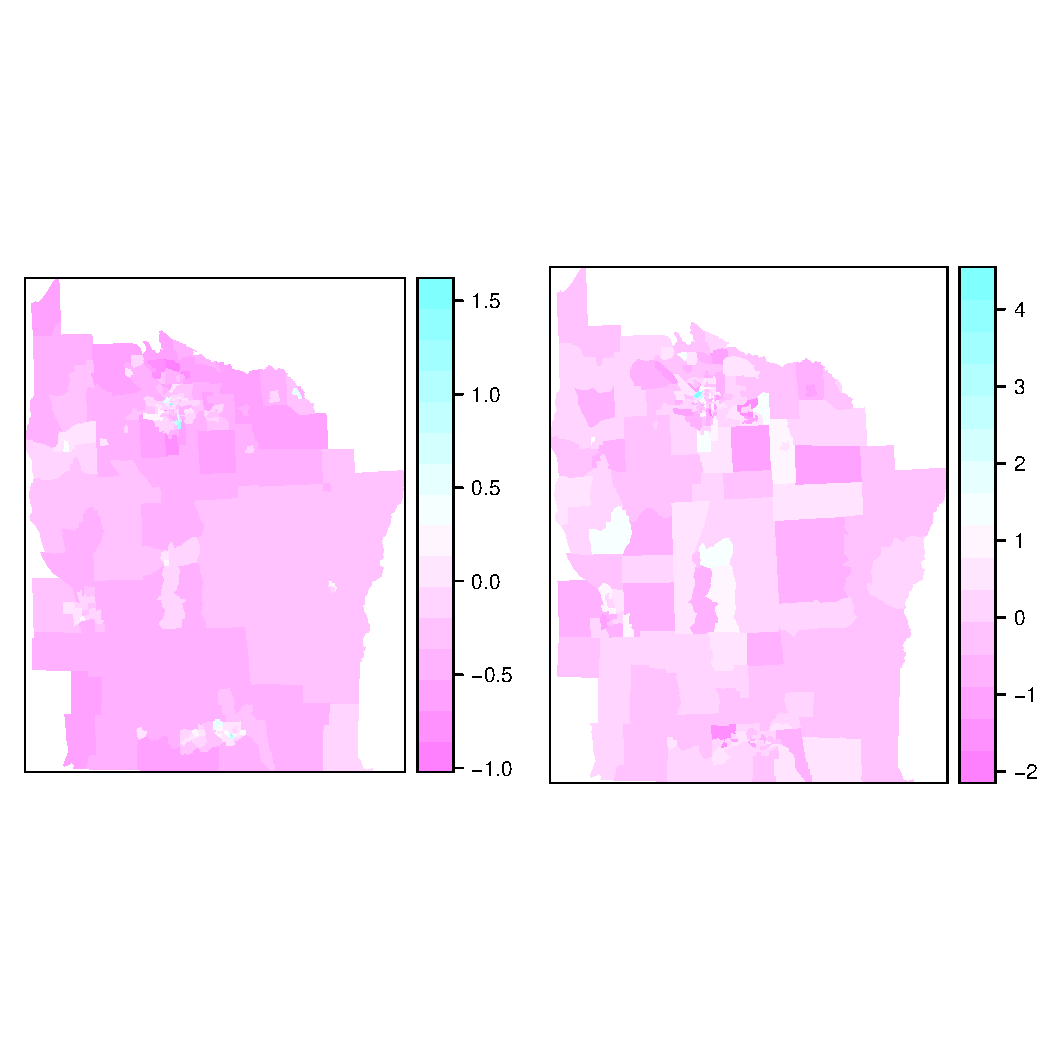
\includegraphics[width=\maxwidth]{figure/unnamed-chunk-16} 

\end{knitrout}

Let's move to a more sophisticated autoregressive model:
$$
 (I - \lambda W)(Y- X\beta) = \varepsilon
$$

In order to specify such a model, we need to create the adjacency matrix $W$. We generate this as a 'spatial weight object' from the neighbor list object we loaded.

\begin{knitrout}
\definecolor{shadecolor}{rgb}{0.969, 0.969, 0.969}\color{fgcolor}\begin{kframe}
\begin{alltt}
\hlcom{# generate weight object from neighbor list object}
\hlcom{# "B" - generates binary weights}
\hlstd{NYlistw}\hlkwb{<-}\hlkwd{nb2listw}\hlstd{(NY_nb,} \hlkwc{style} \hlstd{=} \hlstr{"B"}\hlstd{)}

\hlcom{# fit model (I - lambda* W)(Y- X* beta) = epsilon}
\hlstd{nysar}\hlkwb{<-}\hlkwd{spautolm}\hlstd{(Z}\hlopt{~}\hlstd{PEXPOSURE}\hlopt{+}\hlstd{PCTAGE65P}\hlopt{+}\hlstd{PCTOWNHOME,} \hlkwc{data}\hlstd{=NY8,} \hlkwc{listw}\hlstd{=NYlistw)}

\hlkwd{summary}\hlstd{(nysar)}
\end{alltt}
\begin{verbatim}
## 
## Call: 
## spautolm(formula = Z ~ PEXPOSURE + PCTAGE65P + PCTOWNHOME, data = NY8, 
##     listw = NYlistw)
## 
## Residuals:
##      Min       1Q   Median       3Q      Max 
## -1.56754 -0.38239 -0.02643  0.33109  4.01219 
## 
## Coefficients: 
##              Estimate Std. Error z value
## (Intercept) -0.618193   0.176784 -3.4969
## PEXPOSURE    0.071014   0.042051  1.6888
## PCTAGE65P    3.754200   0.624722  6.0094
## PCTOWNHOME  -0.419890   0.191329 -2.1946
##              Pr(>|z|)
## (Intercept) 0.0004707
## PEXPOSURE   0.0912635
## PCTAGE65P   1.862e-09
## PCTOWNHOME  0.0281930
## 
## Lambda: 0.04049 LR test value: 5.244 p-value: 0.022026 
## Numerical Hessian standard error of lambda: 0.01718 
## 
## Log likelihood: -276.1 
## ML residual variance (sigma squared): 0.4139, (sigma: 0.6433)
## Number of observations: 281 
## Number of parameters estimated: 6 
## AIC: 564.2
\end{verbatim}
\end{kframe}
\end{knitrout}


Note: lambda significantly different from 0 indicates that there is significant reduction in RSS by modelling the spatial correlations.

For more understanding, let's plot the trend and stochastic component, which are the first and second element on the RHS of the following equation:

$$
 Y =  X* \beta + \lambda W)(Y-X\beta) +  \varepsilon
$$

\begin{knitrout}
\definecolor{shadecolor}{rgb}{0.969, 0.969, 0.969}\color{fgcolor}\begin{kframe}
\begin{alltt}
\hlcom{#plot trend and stochastic component}
\hlstd{NY8}\hlopt{$}\hlstd{sar_trend} \hlkwb{<-} \hlstd{nysar}\hlopt{$}\hlstd{fit}\hlopt{$}\hlstd{signal_trend}
\hlstd{NY8}\hlopt{$}\hlstd{sar_stochastic} \hlkwb{<-} \hlstd{nysar}\hlopt{$}\hlstd{fit}\hlopt{$}\hlstd{signal_stochastic}
\hlstd{rds} \hlkwb{<-} \hlkwd{colorRampPalette}\hlstd{(}\hlkwd{brewer.pal}\hlstd{(}\hlnum{8}\hlstd{,} \hlstr{"RdBu"}\hlstd{))}
\hlstd{tr_at} \hlkwb{<-} \hlkwd{seq}\hlstd{(}\hlopt{-}\hlnum{1}\hlstd{,} \hlnum{1.3}\hlstd{,} \hlkwc{length.out}\hlstd{=}\hlnum{21}\hlstd{)}
\hlstd{tr_rds} \hlkwb{<-} \hlkwd{rds}\hlstd{(}\hlkwd{sum}\hlstd{(tr_at} \hlopt{>=} \hlnum{0}\hlstd{)}\hlopt{*}\hlnum{2}\hlstd{)[}\hlopt{-}\hlstd{(}\hlnum{1}\hlopt{:}\hlstd{(}\hlkwd{sum}\hlstd{(tr_at} \hlopt{>=} \hlnum{0}\hlstd{)}\hlopt{-}\hlkwd{sum}\hlstd{(tr_at} \hlopt{<} \hlnum{0}\hlstd{)))]}
\hlstd{tr_pl} \hlkwb{<-} \hlkwd{spplot}\hlstd{(NY8,} \hlkwd{c}\hlstd{(}\hlstr{"sar_trend"}\hlstd{),} \hlkwc{at}\hlstd{=tr_at,} \hlkwc{col}\hlstd{=}\hlstr{"transparent"}\hlstd{,}
                \hlkwc{col.regions}\hlstd{=tr_rds,} \hlkwc{main}\hlstd{=}\hlkwd{list}\hlstd{(}\hlkwc{label}\hlstd{=}\hlstr{"Trend"}\hlstd{,} \hlkwc{cex}\hlstd{=}\hlnum{0.8}\hlstd{))}
\hlstd{st_at} \hlkwb{<-} \hlkwd{seq}\hlstd{(}\hlopt{-}\hlnum{0.16}\hlstd{,} \hlnum{0.39}\hlstd{,} \hlkwc{length.out}\hlstd{=}\hlnum{21}\hlstd{)}
\hlstd{st_rds} \hlkwb{<-} \hlkwd{rds}\hlstd{(}\hlkwd{sum}\hlstd{(st_at} \hlopt{>=} \hlnum{0}\hlstd{)}\hlopt{*}\hlnum{2}\hlstd{)[}\hlopt{-}\hlstd{(}\hlnum{1}\hlopt{:}\hlstd{(}\hlkwd{sum}\hlstd{(st_at} \hlopt{>=} \hlnum{0}\hlstd{)}\hlopt{-}\hlkwd{sum}\hlstd{(st_at} \hlopt{<} \hlnum{0}\hlstd{)))]}
\hlstd{st_pl} \hlkwb{<-} \hlkwd{spplot}\hlstd{(NY8,} \hlkwd{c}\hlstd{(}\hlstr{"sar_stochastic"}\hlstd{),} \hlkwc{at}\hlstd{=st_at,} \hlkwc{col}\hlstd{=}\hlstr{"transparent"}\hlstd{,}
                \hlkwc{col.regions}\hlstd{=st_rds,} \hlkwc{main}\hlstd{=}\hlkwd{list}\hlstd{(}\hlkwc{label}\hlstd{=}\hlstr{"Stochastic"}\hlstd{,} \hlkwc{cex}\hlstd{=}\hlnum{0.8}\hlstd{))}
\hlkwd{plot}\hlstd{(tr_pl,} \hlkwc{split}\hlstd{=}\hlkwd{c}\hlstd{(}\hlnum{1}\hlstd{,}\hlnum{1}\hlstd{,}\hlnum{2}\hlstd{,}\hlnum{1}\hlstd{),} \hlkwc{more}\hlstd{=}\hlnum{TRUE}\hlstd{)}
\hlkwd{plot}\hlstd{(st_pl,} \hlkwc{split}\hlstd{=}\hlkwd{c}\hlstd{(}\hlnum{2}\hlstd{,}\hlnum{1}\hlstd{,}\hlnum{2}\hlstd{,}\hlnum{1}\hlstd{),} \hlkwc{more}\hlstd{=}\hlnum{FALSE}\hlstd{)}
\end{alltt}
\end{kframe}
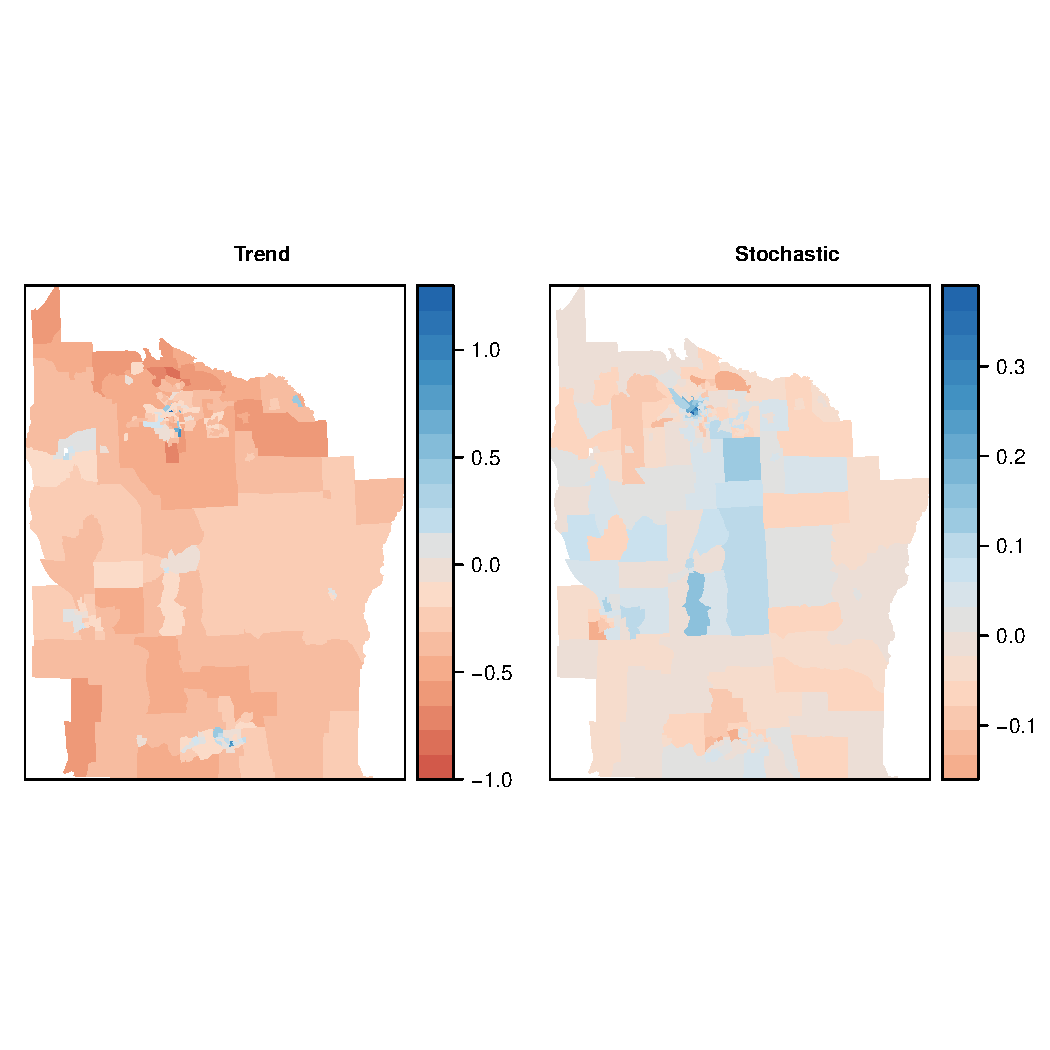
\includegraphics[width=\maxwidth]{figure/unnamed-chunk-18} 

\end{knitrout}

Ok this is great, but how do I transform my data into spatial format? Let's examine how to create spatial data.

There are two important structures,  \verb+"SpatialPointsDataFrame"+ and \verb+listw+.

\begin{knitrout}
\definecolor{shadecolor}{rgb}{0.969, 0.969, 0.969}\color{fgcolor}\begin{kframe}
\begin{alltt}
\hlcom{#Key data type #1: "SpatialPointsDataFrame"}
\hlkwd{getClass}\hlstd{(}\hlstr{"SpatialPointsDataFrame"}\hlstd{)}
\end{alltt}
\begin{verbatim}
## Class "SpatialPointsDataFrame" [package "sp"]
## 
## Slots:
##                                           
## Name:         data  coords.nrs      coords
## Class:  data.frame     numeric      matrix
##                               
## Name:         bbox proj4string
## Class:      matrix         CRS
## 
## Extends: 
## Class "SpatialPoints", directly
## Class "Spatial", by class "SpatialPoints", distance 2
## 
## Known Subclasses: 
## Class "SpatialPixelsDataFrame", directly, with explicit coerce
\end{verbatim}
\begin{alltt}
\hlcom{#read data matrix}
\hlstd{CRAN_df} \hlkwb{<-} \hlkwd{read.table}\hlstd{(}\hlstr{"CRAN051001a.txt"}\hlstd{,} \hlkwc{header}\hlstd{=}\hlnum{TRUE}\hlstd{)}
\hlstd{CRAN_mat} \hlkwb{<-} \hlkwd{cbind}\hlstd{(CRAN_df}\hlopt{$}\hlstd{long, CRAN_df}\hlopt{$}\hlstd{lat)}
\hlkwd{row.names}\hlstd{(CRAN_mat)} \hlkwb{<-} \hlnum{1}\hlopt{:}\hlkwd{nrow}\hlstd{(CRAN_mat)}
\hlkwd{str}\hlstd{(CRAN_mat)}
\end{alltt}
\begin{verbatim}
##  num [1:54, 1:2] 153 145 16.3 -49.3 -42.9 ...
##  - attr(*, "dimnames")=List of 2
##   ..$ : chr [1:54] "1" "2" "3" "4" ...
##   ..$ : NULL
\end{verbatim}
\begin{alltt}
\hlcom{#set CRS }
\hlstd{llCRS} \hlkwb{<-} \hlkwd{CRS}\hlstd{(}\hlstr{"+proj=longlat +ellps=WGS84"}\hlstd{)}
\hlstd{CRAN_sp} \hlkwb{<-} \hlkwd{SpatialPoints}\hlstd{(CRAN_mat,} \hlkwc{proj4string}\hlstd{=llCRS)}
\hlkwd{summary}\hlstd{(CRAN_sp)}
\end{alltt}
\begin{verbatim}
## Object of class SpatialPoints
## Coordinates:
##               min    max
## coords.x1 -122.95 153.03
## coords.x2  -37.82  57.05
## Is projected: FALSE 
## proj4string : [+proj=longlat +ellps=WGS84]
## Number of points: 54
\end{verbatim}
\begin{alltt}
\hlcom{#if you don't need CRS}
\hlstd{llCRS} \hlkwb{<-} \hlkwd{CRS}\hlstd{(}\hlkwd{as.character}\hlstd{(}\hlnum{NA}\hlstd{))}

\hlstd{CRAN_spdf} \hlkwb{<-} \hlkwd{SpatialPointsDataFrame}\hlstd{(CRAN_sp, CRAN_df)}
\hlkwd{summary}\hlstd{(CRAN_spdf)}
\end{alltt}
\begin{verbatim}
## Object of class SpatialPointsDataFrame
## Coordinates:
##               min    max
## coords.x1 -122.95 153.03
## coords.x2  -37.82  57.05
## Is projected: FALSE 
## proj4string : [+proj=longlat +ellps=WGS84]
## Number of points: 54
## Data attributes:
##             place        north          east   
##  Bern          : 2   40d26'N: 2   13d22'E : 2  
##  Pittsburgh, PA: 2   46d57'N: 2   7d26'E  : 2  
##  Aalborg       : 1   20d45'S: 1   80d0'W  : 2  
##  Aizu          : 1   22d43'S: 1   0d10'W  : 1  
##  Ames, IA      : 1   22d54'S: 1   118d15'W: 1  
##  Arezzo        : 1   23d32'S: 1   118d47'E: 1  
##  (Other)       :46   (Other):46   (Other) :45  
##           loc          long        
##  Brazil     : 5   Min.   :-122.95  
##  Germany    : 5   1st Qu.: -47.38  
##  Italy      : 4   Median :   7.85  
##  France     : 3   Mean   :  -0.66  
##  Switzerland: 3   3rd Qu.:  16.83  
##  Australia  : 2   Max.   : 153.03  
##  (Other)    :32                    
##       lat       
##  Min.   :-37.8  
##  1st Qu.: 34.5  
##  Median : 42.7  
##  Mean   : 31.7  
##  3rd Qu.: 47.6  
##  Max.   : 57.0  
## 
\end{verbatim}
\end{kframe}
\end{knitrout}

The second key data type is the class of Spatial Weights - listw. 

It is based on the Spatial neighbors \verb+("nb")+ class. This class is a list of length $n$, where $n$ is the number of our nodes, 
with the index numbers of neighbors of each component stored as an integer vector. Run the following: \verb+vignette("nb", package = "spdep")+ to read more on neighbors.

Recall that we already have \verb+NY_nb+ as an object of nb class. 

On top of it we can add nonzero weights for each pair of neighbors, getting the listw class. 

\begin{knitrout}
\definecolor{shadecolor}{rgb}{0.969, 0.969, 0.969}\color{fgcolor}\begin{kframe}
\begin{alltt}
\hlstd{NY_w} \hlkwb{<-}\hlkwd{nb2listw}\hlstd{(NY_nb)}
\hlkwd{summary}\hlstd{(NY_w)}
\end{alltt}
\begin{verbatim}
## Characteristics of weights list object:
## Neighbour list object:
## Number of regions: 281 
## Number of nonzero links: 1522 
## Percentage nonzero weights: 1.928 
## Average number of links: 5.416 
## Link number distribution:
## 
##  1  2  3  4  5  6  7  8  9 10 11 
##  6 11 28 45 59 49 45 23 10  3  2 
## 6 least connected regions:
## 55 97 100 101 244 245 with 1 link
## 2 most connected regions:
## 34 82 with 11 links
## 
## Weights style: W 
## Weights constants summary:
##     n    nn  S0    S1   S2
## W 281 78961 281 115.4 1169
\end{verbatim}
\end{kframe}
\end{knitrout}

By default each node is normalized to have total sum of out-weights equal to 1. We can also choose to use binary weights.

\begin{knitrout}
\definecolor{shadecolor}{rgb}{0.969, 0.969, 0.969}\color{fgcolor}\begin{kframe}
\begin{alltt}
\hlstd{NY_w} \hlkwb{<-}\hlkwd{nb2listw}\hlstd{(NY_nb,} \hlkwc{style} \hlstd{=} \hlstr{"B"}\hlstd{)}
\hlkwd{summary}\hlstd{(NY_w)}
\end{alltt}
\begin{verbatim}
## Characteristics of weights list object:
## Neighbour list object:
## Number of regions: 281 
## Number of nonzero links: 1522 
## Percentage nonzero weights: 1.928 
## Average number of links: 5.416 
## Link number distribution:
## 
##  1  2  3  4  5  6  7  8  9 10 11 
##  6 11 28 45 59 49 45 23 10  3  2 
## 6 least connected regions:
## 55 97 100 101 244 245 with 1 link
## 2 most connected regions:
## 34 82 with 11 links
## 
## Weights style: B 
## Weights constants summary:
##     n    nn   S0   S1    S2
## B 281 78961 1522 3044 37160
\end{verbatim}
\end{kframe}
\end{knitrout}

\end{document}
